% !TEX root = ../main.tex
\documentclass[../main.tex]{subfiles}

\begin{document}
\section{NPN-Transistor als Schalter \textit{level-shift}}

\subsection{Ziel}

Von einem Mikrocontrollersystem mit $V_{CC} = \SI{3.3}{\volt}$ soll mit Hilfe eines \textit{BC548B}-Transistors eine Schaltung dimensioniert werden, die die Logischen Signale auf ein $V_{CC} = \SI{5}{\volt}$ System überträgt.

Analysiert werden soll die Transferkennlinie und die Aufstiegs- und Abfallzeiten. Zudem soll der Einfluss der kapazitiven Belastung der Schaltung auf die Zeiten der Pegelwechsel aufgezeigt werden.

\subsection{Berechnungen}

Die \textit{Open-Collector-Schaltung} wird mit einem Pull-Up-Widerstand von $R_2 = \SI{1}{\kilo\ohm}$ versehen. $\SI{1}{\kilo\ohm}$ ist ein Standard-Wert, der oft als Pull-Up-Widerstand verwendet wird. Der maximale Kollektrostrom beträgt somit $I_C = \frac{U_s}{R_2} = \frac{\SI{5}{\volt}}{\SI{1}{\kilo\ohm}} = \SI{5}{\milli\ampere}$ und daraus folgt über Gleichung \ref{equ:lsbjt_R1} ein Vorwiderstand von $R_1 = \SI{33}{\kilo\ohm}$

\begin{equation}
    R_1 = \frac{U_{IN} - U_{BE_{max}}}{\frac{I_{C_{max}}}{h_{FE_{min}}} {"u}} = \frac{\SI{3.3}{\volt} - \SI{0.77}{\volt}}{\frac{\SI{5}{\milli\ampere}}{200}3} = \SI{33.7}{\kilo\ohm} \Rightarrow \textrm{E12-Reihe } R_{1} = \SI{33}{\kilo\ohm}
    \label{equ:lsbjt_R1}
\end{equation}

\newpage

\subsection{Messschaltung}

\begin{figure}[h]
    \centering
    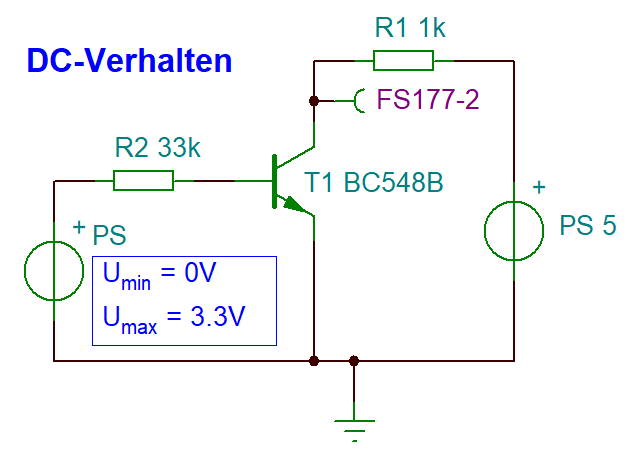
\includegraphics[scale=0.35]{assets/task3_square/messschaltung_task3_DC.PNG}
    \caption{DC-Verhalten Messschaltung}
    \label{fig:circuit_voltage_stabilization_dc}
\end{figure}

\begin{figure}[h]
    \centering
    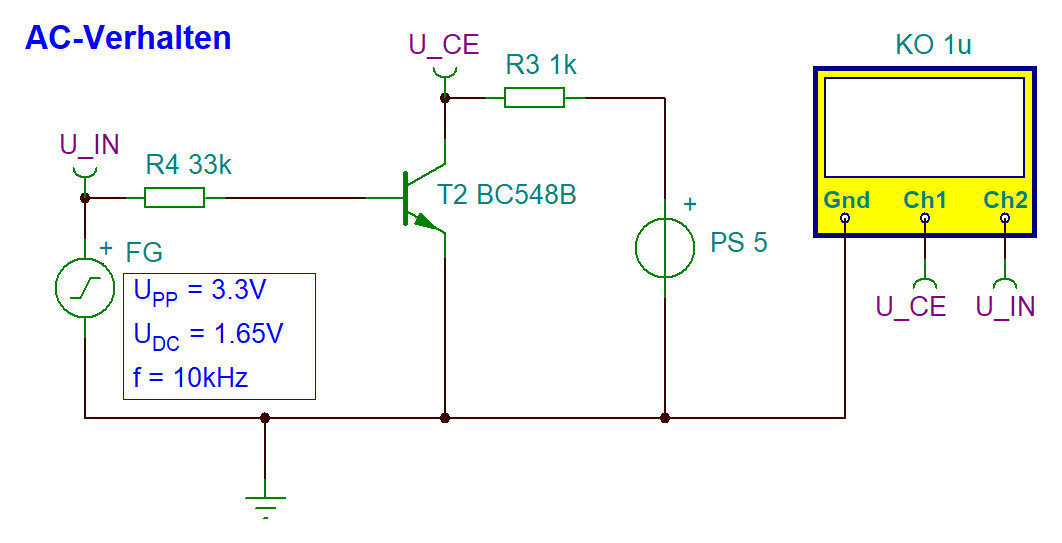
\includegraphics[scale=0.35]{assets/task3_square/messschaltung_task3_AC.PNG}
    \caption{AC-Verhalten Messschaltung}
    \label{fig:circuit_voltage_stabilization_ac}
\end{figure}

\begin{figure}[h]
    \centering
    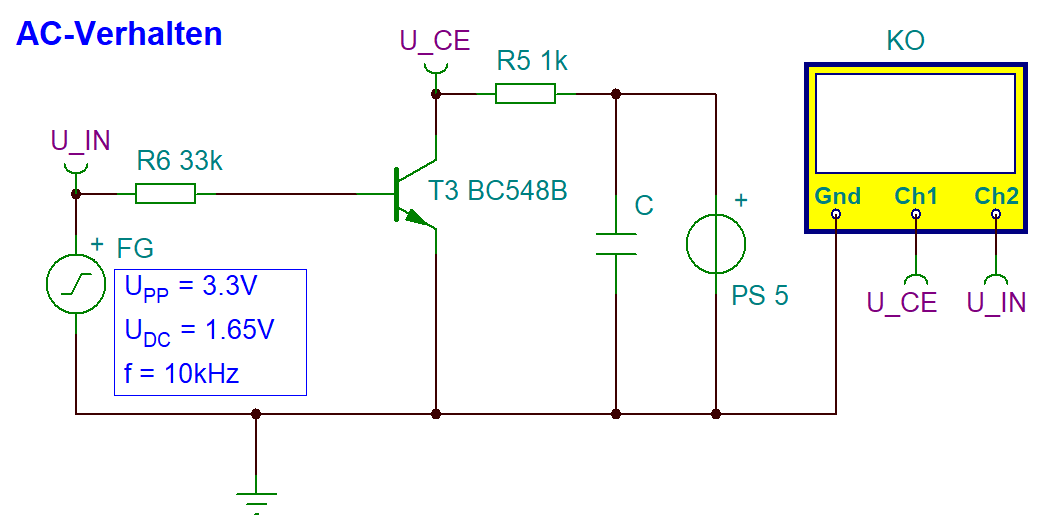
\includegraphics[scale=0.35]{assets/task3_square/messschaltung_task3_AC_capacitor.PNG}
    \caption{AC-Verhalten Messschaltung mit Lastkondensator}
    \label{fig:circuit_voltage_stabilization_ac_cap}
\end{figure}

\newpage

\subsection{Resultate}

\subsubsection{DC-Verhalten}

$U_{OUT}$ entspricht der gemessenen Spannung $U_{CE}$ von der Messschaltung. Der Verstärkungsfaktor $A$ wurde mit folgender Formel berechnet, welche von der Aufgabenbeschreibung entnommen wurde:

\begin{equation}
    A = \frac{\Delta U_{OUT}}{\Delta U_{IN}} 
\end{equation}

\begin{figure}[h]
    \centering
    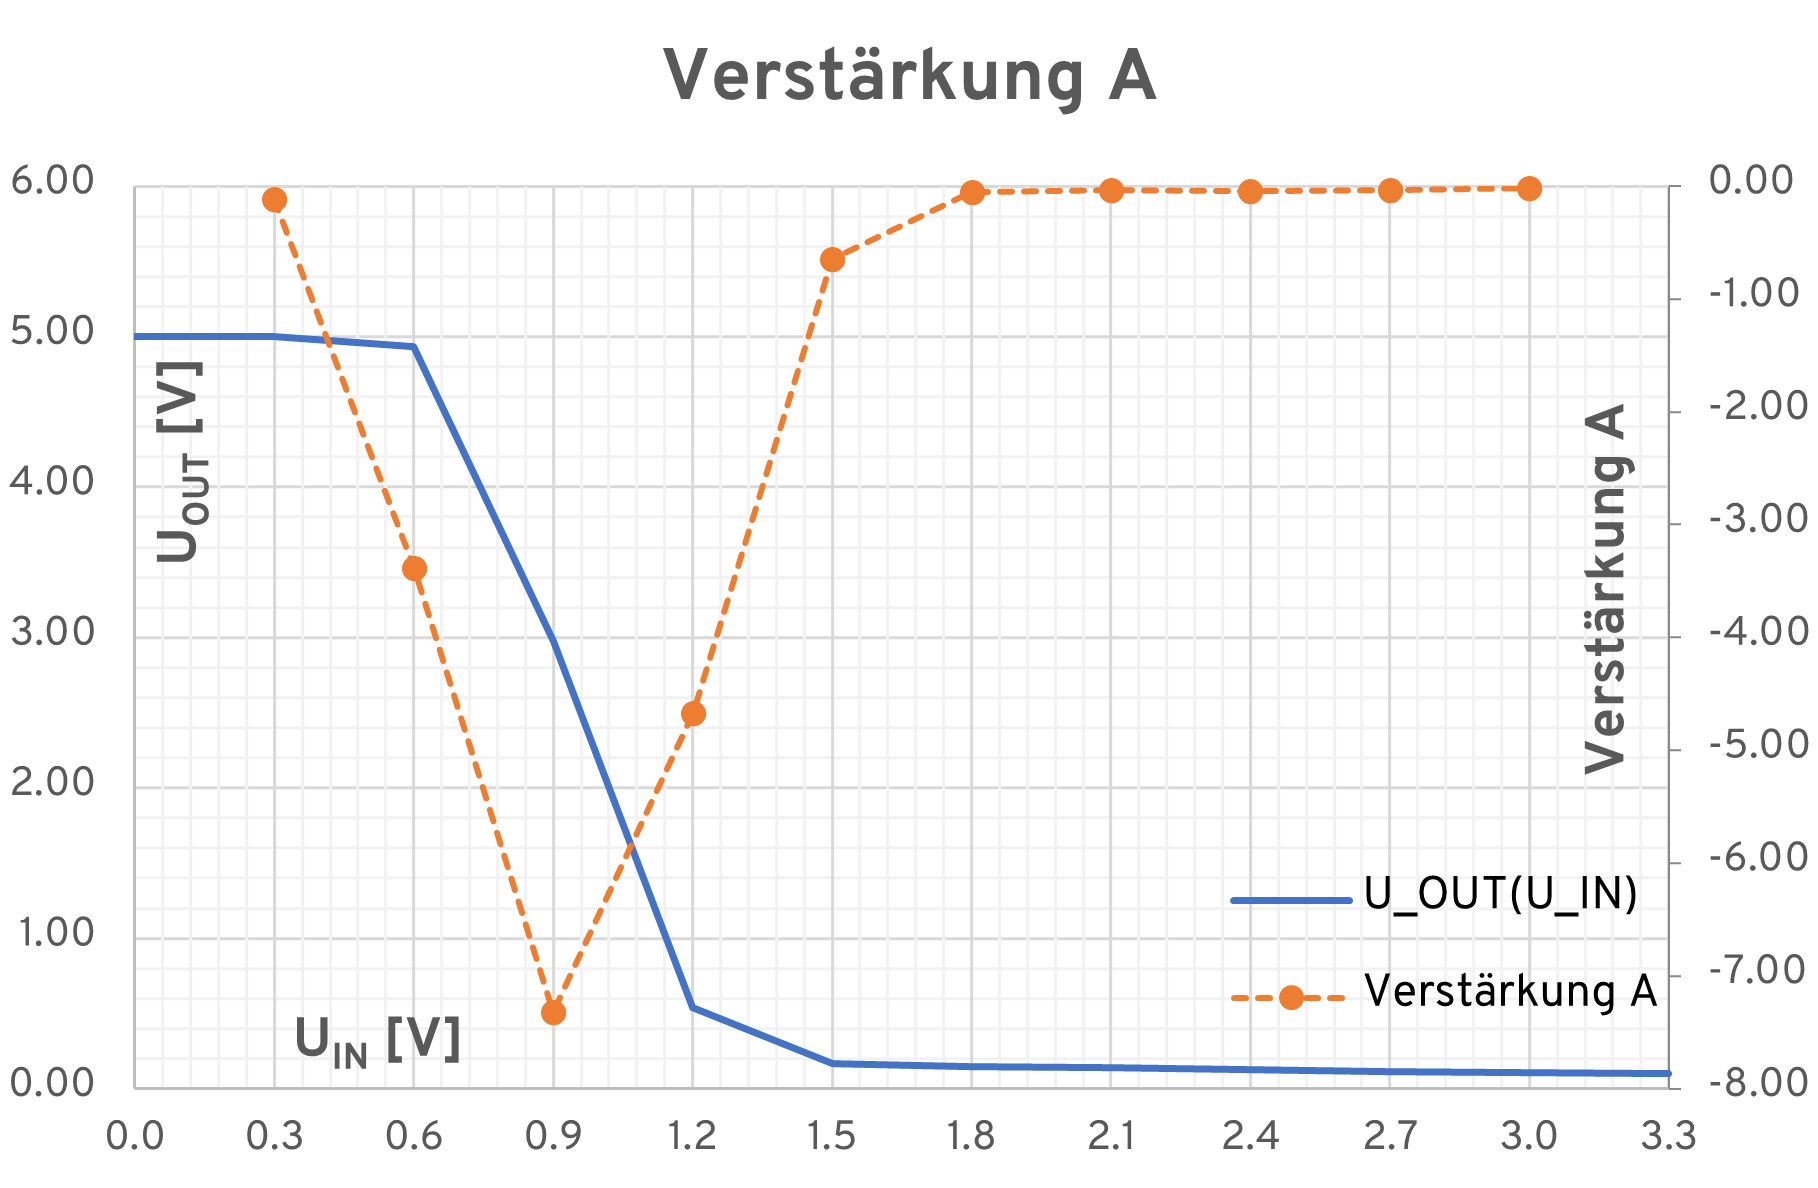
\includegraphics{assets/task3_square/DC_Verhalten Werte.png}
    \caption{Resultate des DC-Verhaltens}
    \label{fig:result_dc_behaviour}
\end{figure}

\subsubsection{AC-Verhalten}

\begin{figure}[h]
    \centering
    \begin{subfigure}[b]{0.45\textwidth}
        \centering
        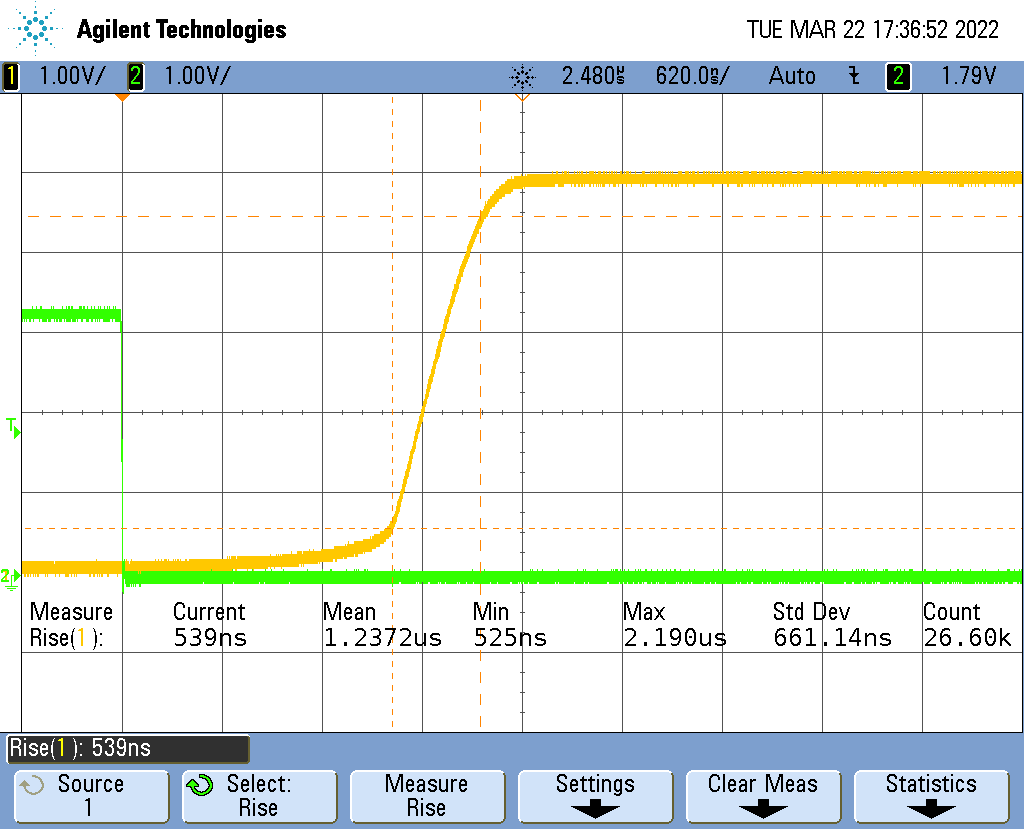
\includegraphics[width=\textwidth]{assets/task3_square/SquareRise_0F.png}
        \caption{Rise-Time ($\SI{539}{\nano\seconds}$)}
        \label{fig:square_rise}
    \end{subfigure}
    \hfill
    \begin{subfigure}[b]{0.45\textwidth}
        \centering
        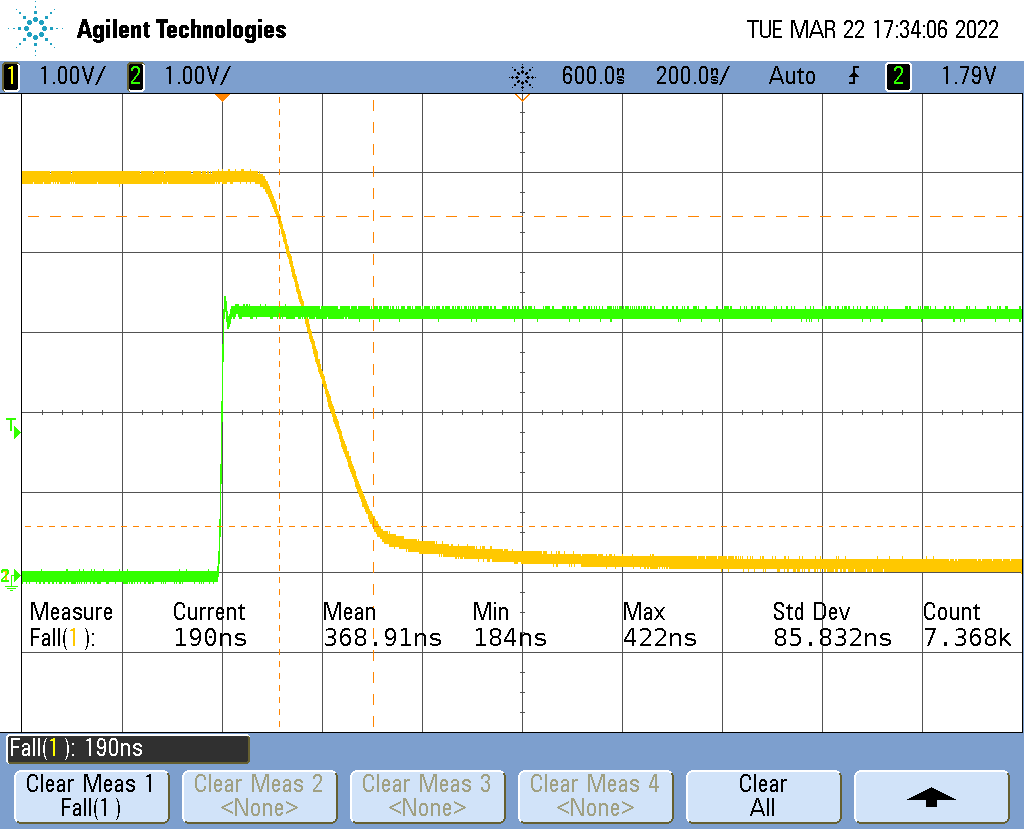
\includegraphics[width=\textwidth]{assets/task3_square/SquareFall_0F.png}
        \caption{Fall-Time ($\SI{198}{\nano\seconds}$)}
        \label{fig:square_fall}
    \end{subfigure}
    \caption{Messresultate ohne Kapazität}
    \label{fig:square_no_cap}
\end{figure}

\newpage

\begin{figure}[h]
    \centering
    \begin{subfigure}[b]{0.45\textwidth}
        \centering
        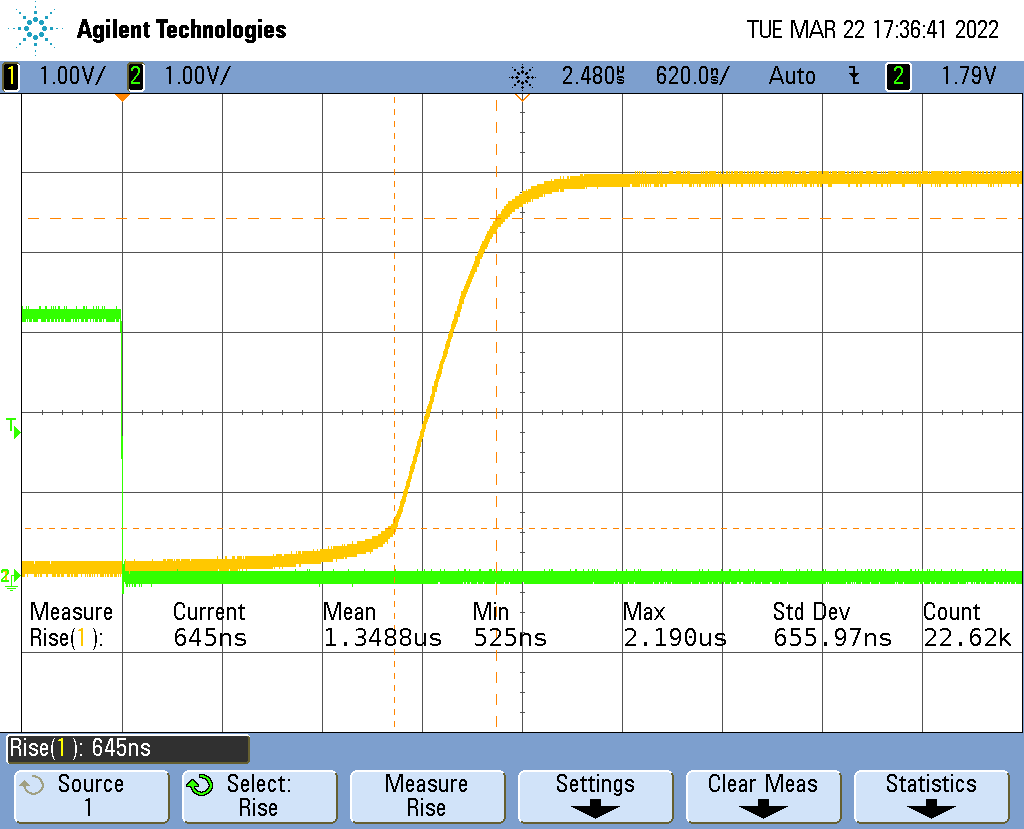
\includegraphics[width=\textwidth]{assets/task3_square/SquareRise_100pF.png}
        \caption{Rise-Time ($\SI{645}{\nano\seconds}$)}
        \label{fig:square_rise}
    \end{subfigure}
    \hfill
    \begin{subfigure}[b]{0.45\textwidth}
        \centering
        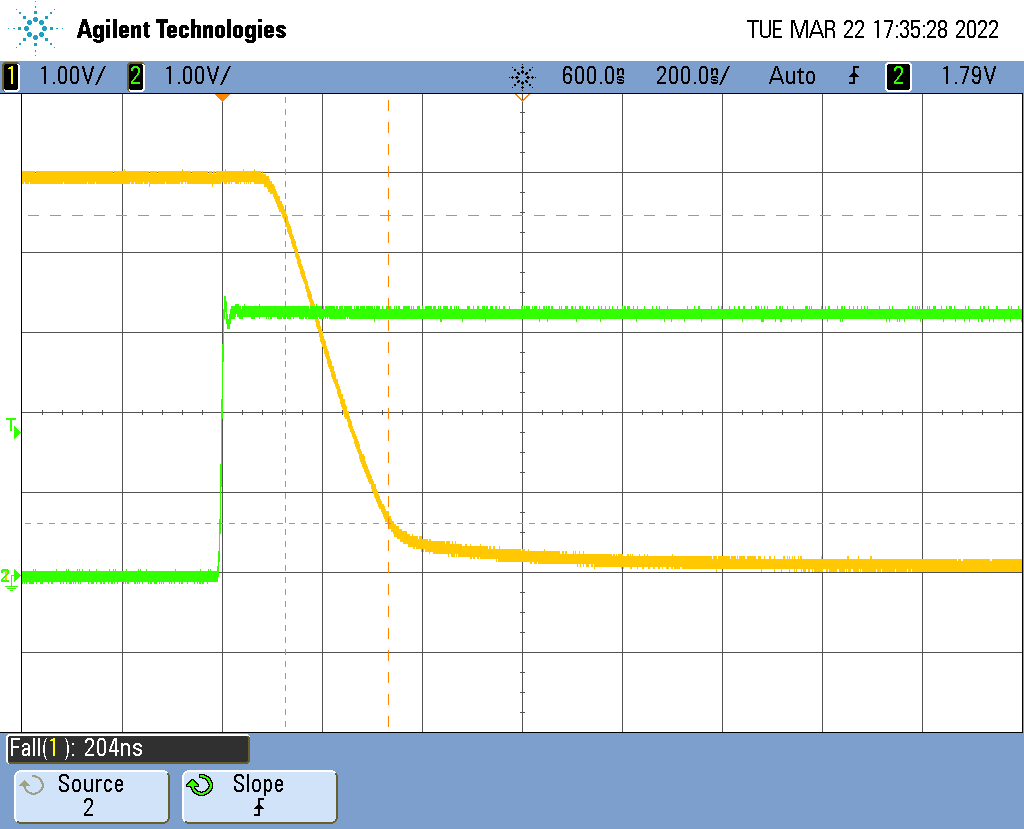
\includegraphics[width=\textwidth]{assets/task3_square/SquareFall_100pF.png}
        \caption{Fall-Time ($\approx\SI{200}{\nano\seconds}$)}
        \label{fig:square_fall}
    \end{subfigure}
    \caption{Messresultate mit $\SI{100}{\pico\farad}$ Kapazität}
    \label{fig:square_no_cap}
\end{figure}

\begin{figure}[h]
    \centering
    \begin{subfigure}[b]{0.45\textwidth}
        \centering
        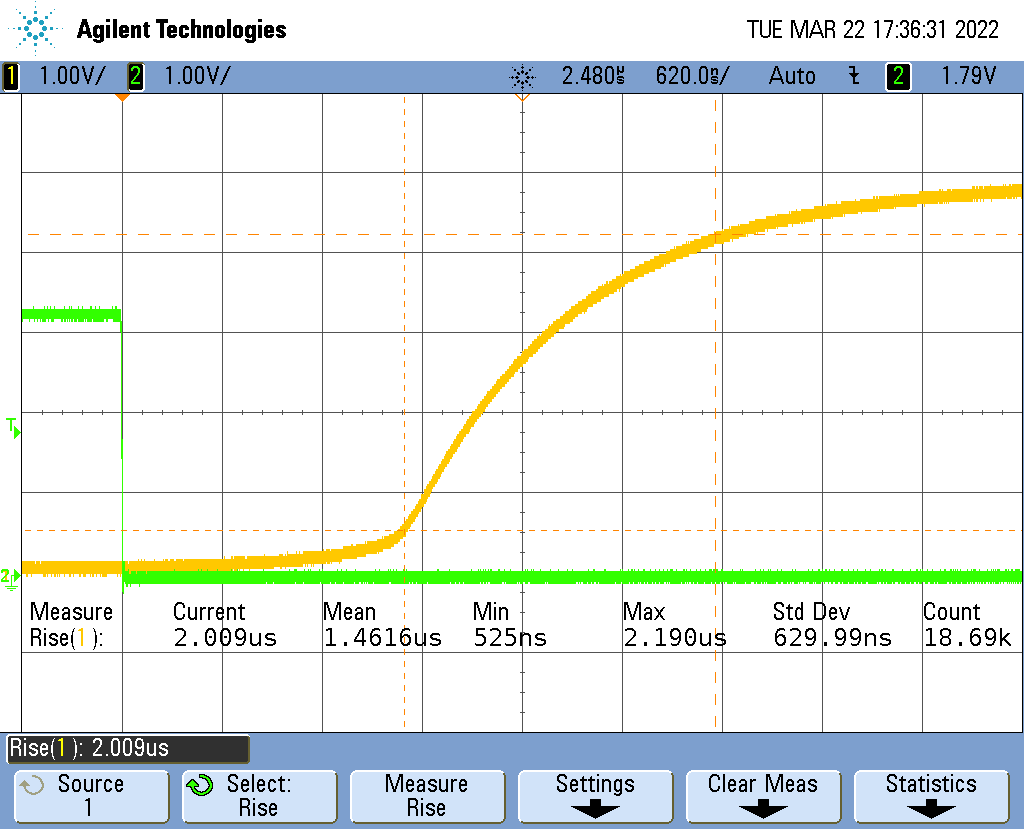
\includegraphics[width=\textwidth]{assets/task3_square/SquareRise_1nF.png}
        \caption{Rise-Time ($\SI{2.009}{\micro\seconds}$)}
        \label{fig:square_rise}
    \end{subfigure}
    \hfill
    \begin{subfigure}[b]{0.45\textwidth}
        \centering
        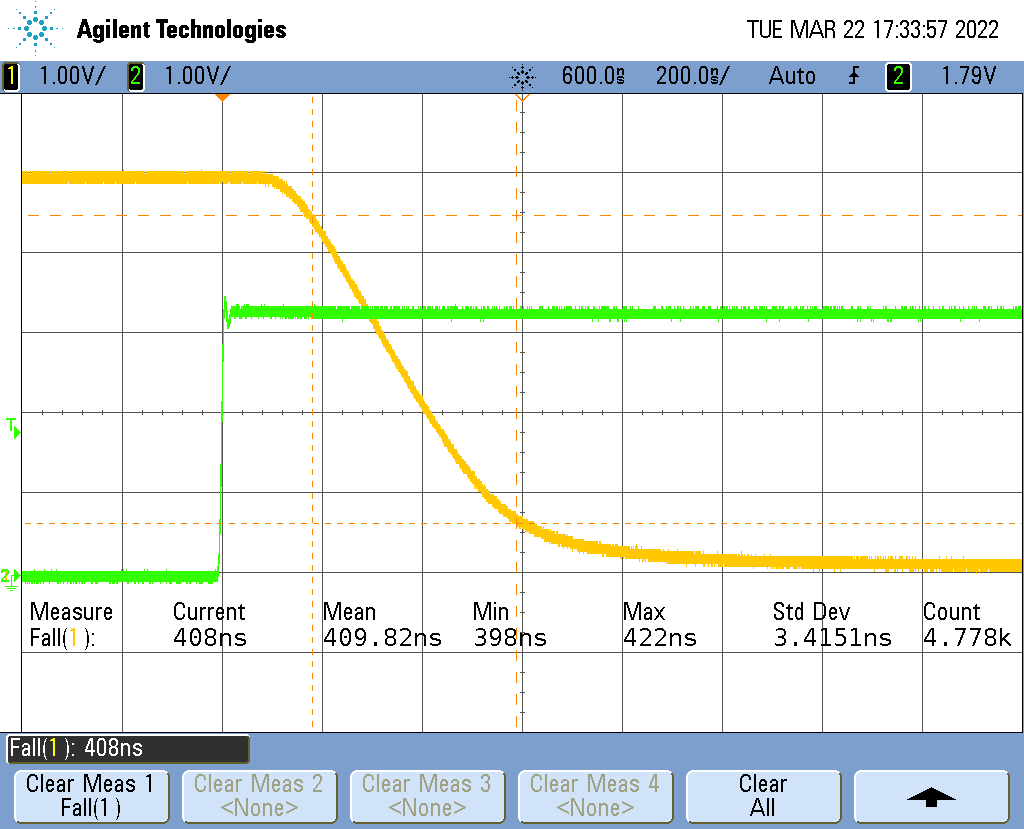
\includegraphics[width=\textwidth]{assets/task3_square/SquareFall_1nF.png}
        \caption{Fall-Time ($\SI{408}{\nano\seconds}$)}
        \label{fig:square_fall}
    \end{subfigure}
    \caption{Messresultate mit $\SI{1}{\nano\farad}$ Kapazität}
    \label{fig:square_no_cap}
\end{figure}

\subsection{Schlussfolgerung}

In der Abbildung \ref{fig:result_dc_behaviour} der DC-Verhaltens-Messung kann im Bereich von $\SI{0.6}{\volt}$ und $\SI{1.2}{\volt}$ einen starken Abfall von ungefähr $-7.3$ erkannt werden. Nachdem $U_{IN}$ die Sättigungsspannung $U_{BE(on)}$ überschritten hat, welche nach Datenblatt ungefähr $\SI{0.7}{\volt}$ beträgt, nähert sich die Spannung $U_{CE}$ dem Wert $\SI{100}{\milli\volt}$. Der Grund ist die Erreichung der Sättigungsspannung zwischen Basis und Emitter.

Beim AC-Verhalten zeigen die verschiedenen Kapazitäten unterschiedliche Anstiegs- und Abfallzeiten, wobei diese Zeiten träger wurden, wenn die Lastkapazitäten grösser wurden. Wird die lastlose Messung mit der $\SI{1}{\nano\farad}$-Messung verglichen, kann eine Verzögerung erkannt werden.

\end{document}